\documentclass[a4paper,11pt]{exam}
\usepackage[utf8]{inputenc}
\usepackage{enumerate}

\date{November 5, 2018}
\title{RE355 - Introduction to Cloud Networking \\
Lab session 2: \textit{Dockerizing} Distributed Applications}
\author{Simon Da Silva \and Mathias Lacaud}

%\usepackage{fancyhdr}
\usepackage{listings}
\usepackage{graphicx}
\usepackage{hyperref}

%\pagestyle{fancy}
%\fancyhf{}
\rhead{Bordeaux INP: ENSEIRB-MATMECA}
\lhead{RE355 - Introduction to Cloud Networking}

\lstset{language=sh,basicstyle=\ttfamily,columns=fullflexible}

\begin{document}

\maketitle

\section{Introduction}

\subsection{Installing docker compose}

Docker and Docker Compose should be already installed. Check that everything works with:

\begin{lstlisting}[frame=single,language={sh}]  % Start your code-block

$ docker-compose -f hello-world-composition.yml up

\end{lstlisting}

\subsection{Basic Introduction to Docker Compose}

This is a quick description of \textit{docker compose}. If you don't know \textit{docker compose}, go through these explanations -- you will use them in the rest of the lab.
This introduction presents a simple web application that has two software components: a front-end written in Python and a MongoDB database.

\subsubsection*{Build images}

\begin{lstlisting}[frame=single,language={sh}]  % Start your code-block

# change directory and build image
$ cd intro/web
$ docker build -t re351/web .

# now the database
$ cd ../database
$ docker build -t re351/data

\end{lstlisting}

Now you can execute the application. The web server is listening on port 8080 and it depends on the database.

\subsubsection*{Executing the app (you should know this)}

\textit{Warning: You really have to use 'data' as the name. Do you know why it is necessary? Remember to kill and remove the containers when you are done playing.}

\begin{lstlisting}[frame=single,language={sh}]  % Start your code-block

$ docker run -d --rm --name data re351/database
$ docker run -d --rm -p 8080:8080 --link data re351/web 
      
\end{lstlisting}

Now you can go to the browser and enjoy this ``awesome'' application.

\subsubsection*{Using docker compose}

Create a new file with the name \textit{docker-compose.yml} under the directory \textit{intro}. Edit it and type the following:

\begin{lstlisting}[frame=single,language={sh}, tabsize=2, numbers=left]  
version: '2'
services:
	web:
		build:
			context: ./web
		image: re351/web:latest
		ports:
		- "8080:8080"
		links:
		- data

	data:
		container_name: data
		build:
			context: ./database
		image: re351/data       
\end{lstlisting}

In this docker compose file we are declaring two containers: \textit{web} (line 3) and \textit{data} (line 12).
They use images \textit{re351/web} and \textit{re351/data}.
In our case, this means using the Docker files inside directories \textit{./web} and \textit{./database}.
As you can see, the there is a port mapping (same as \textit{-p}), and the \textit{web} container is linked to \textit{data}.
Finally, in lines 5 and 15, we specify how to build the images if they don't exists. 

\subsection*{Deploying and stopping the composition}

\begin{lstlisting}[frame=single,language={sh}] % Start your code-block

# no need to speficy the file name. By default it uses docker-compose.yml.
$ docker-compose up

# play time ...

# then you can stop it using Ctrl+C or the command below
$ docker-compose down

\end{lstlisting}

You can use the flag \textit{-d} to launch the composition in detached mode. In such a case, using the \textit{down} subcommand is the only option to stop the composition. 
To see a description of each subcommand simply type:

\begin{lstlisting}[frame=single,language={sh}] % Start your code-block

# list of subcommands
$ docker-compose

# description of one subcommand
$ docker-compose up --help

\end{lstlisting}

\textit{Question}: what ip address is assigned to each container deployed? Are there differences in comparison to using vanilla \textit{docker}?

\subsection{Online documentation}

Additional information on docker compose can be found in the official online documentation~\footnote{https://docs.docker.com/compose/overview/}. Particularly,  in the compose file reference~\footnote{https://docs.docker.com/compose/compose-file/}.

\section{Dockerizing an application}

The idea of this TP is to deploy an application using Docker containers.
Currently, the application cannot be executed using docker. Your job is to ease the deployment of its components by using docker containers.
A high-level view of the applications is depicted in Figure~\ref{fig:architecture}.

\begin{figure}[!ht]
	\centering
	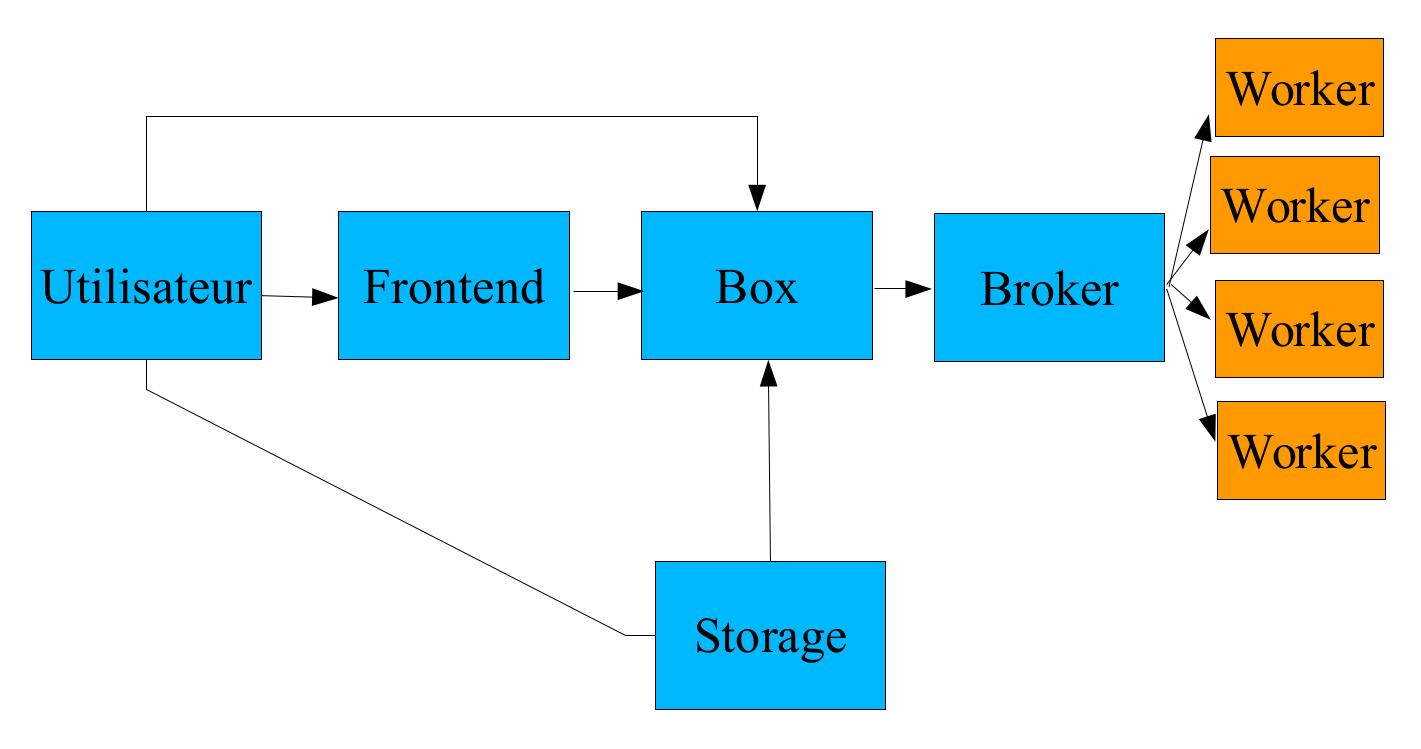
\includegraphics[width=0.8\textwidth]{fig/architecture.png}
	\label{fig:architecture}
\end{figure}

This application has five components that can be deployed in dockers containers.
Your task is to create a docker image for each component and a docker compose file to easily deploy the application.

Along the TP you will use the source code of the application. Clone the \textit{git} repository and \textit{cd} into the cloned directory. 


\subsection{Building images}

\begin{questions}
	\question The \textit{\textbf{Broker}} is simply a RabbitMQ server. Find and image in \textit{Docker Hub}~\footnote{https://hub.docker.com/explore/} and pull it.
	\begin{enumerate}[(a)] % (a)
		\item What is RabbitMQ?
		\item What is the standard port used in RabbitMQ?
		\item Create a \textit{compose} file and define a service ``broker'' based on the rabbitmq image.
	\end{enumerate}	
	
	\question Define a Dockerfile for the \textit{\textbf{frontend}}.
	\begin{enumerate}[(a)] % (a)
		\item What base image can we use?
		\item What tools do you use to install the dependencies?
		\item Add the service to the \textit{compose} file.
		\item What is the error in the application? Can you tell by looking to the source code in the browser?
	\end{enumerate}
	
	\textbf{Hints}:
	\begin{itemize}
		\item Remember that a \textit{Dockerfile} has: base image, dependencies, copy source code, entry point.
		\item The frontend is accessed through port 8080. You can access it using a browser.
		\item The application uses \textit{flask}, a framework for web development in Python.
		\item The server is executed using \textit{python frontend.py http://BoxIpAddr:8081}. Don't worry about the address right now.
	\end{itemize}
	
	\question Now it is time to dockerize the \textit{\textbf{box}}. Jump into the directory \textit{dvd2c-box}. This component is far more complex than the \textit{\textbf{frontend}}. It requires Java 8 and the Maven build system. The component receives requests on port 8081 and uses a MySQL database.
	
	\begin{enumerate}[(a)] % (a)
		\item What base image can we use?
		\item Add the service to the \textit{compose} file.
		\item What are the modifications required in the previously defined services?
		\item Why do we need to start \textit{mysql} in such a way?
		\item How do you force the box to depend on the broker?
		\item Why the box fails during start-up and is not able to access the broker?
	\end{enumerate}
	
	\textbf{Hints}:
	\begin{itemize}
		\item Find the ``right'' base image by searching in Docker Hub. Maven is not the simplest tool to use. However, if the tools are properly installed, compiling is easy:

\begin{lstlisting}[frame=single,language={sh}] %

$ mvn install -Djavax.xml.accessExternalSchema=all \
> -Dmaven.test.skip=true
\end{lstlisting}

		\item For installing MySql:
		
\begin{lstlisting}[frame=single,language={sh}] %

$ export DEBIAN_FRONTEND=noninteractive && apt-get install \
> --yes -q mysql-server
\end{lstlisting}

		\item And an empty MySql database is also needed:

\begin{lstlisting}[frame=single,language={sh}] %	
	
$ service mysql start && mysql -u root -e "create database mediahome;" 
\end{lstlisting}

		\item Finally, this service requires several command line arguments:

\begin{lstlisting}[frame=single,language={sh}] %
		
$ service mysql start && java -jar \
> target/dvd2c-box-0.8.0-jar-with-dependencies.jar \ 
> -i `getent hosts $HOSTNAME | cut -d ' ' -f1` -p 8081 \
> --rabbit-host broker --rabbit-port 5672 --database_url \
> jdbc:mysql://localhost:3306/mediahome --database_username root
\end{lstlisting}

	\end{itemize}
	
	\question Sometimes, an application running within a container must wait until another container is ``ready'' (e.g., the web application of the introduction requires access to the database). However, when \textit{compose} deploys many services they are executed at the same time, without waiting. As a consequence, a container can fail because its dependencies are not ready. In the official documentation a solution is proposed~\footnote{https://docs.docker.com/compose/startup-order/}.
	
		\begin{enumerate}[(a)] % (a)
			\item What is wrong with the proposed solution? How can we reuse it?
			\item Why the application in the introduction doesn't fail?
			\item How should you modify the \textit{\textbf{Box}}'s \textit{dockerfile} to fix this issue?
			\item How should you modify the \textit{\textbf{Frontend}}'s \textit{dockerfile} to fix this issue? Some modification in \textit{docker-compose.yml}?
			
		\end{enumerate}
	
	\question Use file \textit{Dockerfile.worker} to create the worker's image. Afterwards, complete the \textit{composition} and deploy it. You can use the file \textit{trailer\_480p.mov} to answer the following questions:
	
	\begin{enumerate}[(a)] % (a)
		\item After uploading a video file, the results files are stored in which server? 
		\item How many HTTP requests are executed by the browser when you refresh the page? 
	\end{enumerate}
	
	\textbf{Hint:}
	Remember tcpdump is your friend, albeit a complicated one.
	
	\question So far the application has been deployed without a dedicated storage server. Now it is time to remedy such a shortcoming. Let's dockerize the server \textit{store}.
	
	\begin{enumerate}[(a)] % (a)
		\item What base image can we use?
		\item Add the service to the \textit{compose} file.
		\item What are the modifications required in the previously defined services?
		\item What commands we must add to ensure that everything is ready when this container starts?
		\item Test the application and check the URL of the encoded videos? Is it the same as before? 
	\end{enumerate}
\end{questions}

\section{Managing the resources of a cloud-based application}

\begin{questions}
	\question Let's assign some CPU quota to the web application we discuss in the introduction. Go to folder \textit{broken\_introduction} and deploy the application.
	
	\begin{enumerate}[(a)] % (a)
		\item What is the time needed to answer a request when no quota is used?
		\item Set a quota of 25\% of the CPU for the Web Container. What must be added to \textit{composition} file? 
		\item How long does it take to answer a request when the quota is 25\%?
	\end{enumerate}
	
	\question Suppose we have two clients accessing the application \textit{broken\_introduction}. We are offering them the same service but with a different quality. Modify the composition file to deploy a second \textit{web} container with a quota of 75\% of CPU.
	
	\begin{enumerate}[(a)] % (a)
	 	\item How long does it take to update the page? How are you testing this?
	\end{enumerate}
	
	\question We want to expose the previous application using the same URI for both clients (e.g., http://unique-addr:8888/) . This means that client 1 will connect to a service that has a CPU quota of 25\% and client 2 to a service with a quota of 75\%.
	 
	\begin{enumerate}[(a)] % (a)
		\item What tools should we use to achieve this?
		\item What should we modify in the \textit{composition} file?
		\item How can you test this new deployment?
	\end{enumerate}
	
\end{questions}

\end{document}
